
%DIF LATEXDIFF DIFFERENCE FILE
%DIF DEL ICUAS_Main_new.tex   Thu Nov  2 18:28:10 2017
%DIF ADD ICUAS_Main_old.tex   Fri Nov  3 14:15:36 2017
\documentclass[conference]{IEEEtran}
\usepackage[utf8]{inputenc}
\usepackage{graphicx}
\usepackage{amsmath}
\usepackage{amssymb}
\usepackage[version=4]{mhchem}
\usepackage{siunitx}
\usepackage{longtable,tabularx}
\usepackage{listings}
\usepackage{float}
%DIF 12d12
%DIF < 
%DIF -------
%\usepackage{subcaption}
\usepackage{multicol}
\usepackage{dblfloatfix}
\usepackage{color}
\usepackage{subfigure}% subcaptions for subfigures
\usepackage{subfigmat}% matrices of similar subfigures, aka small
%\hyphenation{op-tical net-works semi-conduc-tor}
\usepackage{multirow}
\usepackage[table,xcdraw]{xcolor}
%DIF < \usepackage{soul}
%DIF < 
%DIF < %\floatstyle{boxed}
%DIF < %\restylefloat{figure}
%DIF PREAMBLE EXTENSION ADDED BY LATEXDIFF
%DIF UNDERLINE PREAMBLE %DIF PREAMBLE
\RequirePackage[normalem]{ulem} %DIF PREAMBLE
\RequirePackage{color}\definecolor{RED}{rgb}{1,0,0}\definecolor{BLUE}{rgb}{0,0,1} %DIF PREAMBLE
\providecommand{\DIFadd}[1]{{\protect\color{blue}\uwave{#1}}} %DIF PREAMBLE
\providecommand{\DIFdel}[1]{{\protect\color{red}\sout{#1}}}                      %DIF PREAMBLE
%DIF SAFE PREAMBLE %DIF PREAMBLE
\providecommand{\DIFaddbegin}{} %DIF PREAMBLE
\providecommand{\DIFaddend}{} %DIF PREAMBLE
\providecommand{\DIFdelbegin}{} %DIF PREAMBLE
\providecommand{\DIFdelend}{} %DIF PREAMBLE
%DIF FLOATSAFE PREAMBLE %DIF PREAMBLE
\providecommand{\DIFaddFL}[1]{\DIFadd{#1}} %DIF PREAMBLE
\providecommand{\DIFdelFL}[1]{\DIFdel{#1}} %DIF PREAMBLE
\providecommand{\DIFaddbeginFL}{} %DIF PREAMBLE
\providecommand{\DIFaddendFL}{} %DIF PREAMBLE
\providecommand{\DIFdelbeginFL}{} %DIF PREAMBLE
\providecommand{\DIFdelendFL}{} %DIF PREAMBLE
\newcommand{\DIFscaledelfig}{0.5}
%DIF HIGHLIGHTGRAPHICS PREAMBLE %DIF PREAMBLE
\RequirePackage{settobox} %DIF PREAMBLE
\RequirePackage{letltxmacro} %DIF PREAMBLE
\newsavebox{\DIFdelgraphicsbox} %DIF PREAMBLE
\newlength{\DIFdelgraphicswidth} %DIF PREAMBLE
\newlength{\DIFdelgraphicsheight} %DIF PREAMBLE
% store original definition of \includegraphics %DIF PREAMBLE
\LetLtxMacro{\DIFOincludegraphics}{\includegraphics} %DIF PREAMBLE
\newcommand{\DIFaddincludegraphics}[2][]{{\color{blue}\fbox{\DIFOincludegraphics[#1]{#2}}}} %DIF PREAMBLE
\newcommand{\DIFdelincludegraphics}[2][]{% %DIF PREAMBLE
\sbox{\DIFdelgraphicsbox}{\DIFOincludegraphics[#1]{#2}}% %DIF PREAMBLE
\settoboxwidth{\DIFdelgraphicswidth}{\DIFdelgraphicsbox} %DIF PREAMBLE
\settoboxtotalheight{\DIFdelgraphicsheight}{\DIFdelgraphicsbox} %DIF PREAMBLE
\scalebox{\DIFscaledelfig}{% %DIF PREAMBLE
\parbox[b]{\DIFdelgraphicswidth}{\usebox{\DIFdelgraphicsbox}\\[-\baselineskip] \rule{\DIFdelgraphicswidth}{0em}}\llap{\resizebox{\DIFdelgraphicswidth}{\DIFdelgraphicsheight}{% %DIF PREAMBLE
\setlength{\unitlength}{\DIFdelgraphicswidth}% %DIF PREAMBLE
\begin{picture}(1,1)% %DIF PREAMBLE
\thicklines\linethickness{2pt} %DIF PREAMBLE
{\color[rgb]{1,0,0}\put(0,0){\framebox(1,1){}}}% %DIF PREAMBLE
{\color[rgb]{1,0,0}\put(0,0){\line( 1,1){1}}}% %DIF PREAMBLE
{\color[rgb]{1,0,0}\put(0,1){\line(1,-1){1}}}% %DIF PREAMBLE
\end{picture}% %DIF PREAMBLE
}\hspace*{3pt}}} %DIF PREAMBLE
} %DIF PREAMBLE
\LetLtxMacro{\DIFOaddbegin}{\DIFaddbegin} %DIF PREAMBLE
\LetLtxMacro{\DIFOaddend}{\DIFaddend} %DIF PREAMBLE
\LetLtxMacro{\DIFOdelbegin}{\DIFdelbegin} %DIF PREAMBLE
\LetLtxMacro{\DIFOdelend}{\DIFdelend} %DIF PREAMBLE
\DeclareRobustCommand{\DIFaddbegin}{\DIFOaddbegin \let\includegraphics\DIFaddincludegraphics} %DIF PREAMBLE
\DeclareRobustCommand{\DIFaddend}{\DIFOaddend \let\includegraphics\DIFOincludegraphics} %DIF PREAMBLE
\DeclareRobustCommand{\DIFdelbegin}{\DIFOdelbegin \let\includegraphics\DIFdelincludegraphics} %DIF PREAMBLE
\DeclareRobustCommand{\DIFdelend}{\DIFOaddend \let\includegraphics\DIFOincludegraphics} %DIF PREAMBLE
\LetLtxMacro{\DIFOaddbeginFL}{\DIFaddbeginFL} %DIF PREAMBLE
\LetLtxMacro{\DIFOaddendFL}{\DIFaddendFL} %DIF PREAMBLE
\LetLtxMacro{\DIFOdelbeginFL}{\DIFdelbeginFL} %DIF PREAMBLE
\LetLtxMacro{\DIFOdelendFL}{\DIFdelendFL} %DIF PREAMBLE
\DeclareRobustCommand{\DIFaddbeginFL}{\DIFOaddbeginFL \let\includegraphics\DIFaddincludegraphics} %DIF PREAMBLE
\DeclareRobustCommand{\DIFaddendFL}{\DIFOaddendFL \let\includegraphics\DIFOincludegraphics} %DIF PREAMBLE
\DeclareRobustCommand{\DIFdelbeginFL}{\DIFOdelbeginFL \let\includegraphics\DIFdelincludegraphics} %DIF PREAMBLE
\DeclareRobustCommand{\DIFdelendFL}{\DIFOaddendFL \let\includegraphics\DIFOincludegraphics} %DIF PREAMBLE
%DIF LISTINGS PREAMBLE %DIF PREAMBLE
\lstdefinelanguage{codediff}{ %DIF PREAMBLE
  moredelim=**[is][\color{red}]{*!----}{----!*}, %DIF PREAMBLE
  moredelim=**[is][\color{blue}]{*!++++}{++++!*} %DIF PREAMBLE
} %DIF PREAMBLE
\lstdefinestyle{codediff}{ %DIF PREAMBLE
	belowcaptionskip=.25\baselineskip, %DIF PREAMBLE
	language=codediff, %DIF PREAMBLE
	basicstyle=\ttfamily, %DIF PREAMBLE
	columns=fullflexible, %DIF PREAMBLE
	keepspaces=true, %DIF PREAMBLE
} %DIF PREAMBLE
%DIF END PREAMBLE EXTENSION ADDED BY LATEXDIFF

\begin{document}

\title{\DIFdelbegin \DIFdel{An Intercept and Following Strategy for a Multi-rotor Platform using a Modified Proportional Navigation}\DIFdelend \DIFaddbegin \DIFadd{TITLE}\DIFaddend }

\author{\IEEEauthorblockN{Garrett S. Clem, Jay P. Wilhelm}
\DIFdelbegin %DIFDELCMD < \IEEEauthorblockA{Department of Mechanical Engineering\\
%DIFDELCMD < Ohio University\\
%DIFDELCMD < Athens, Ohio 45701\\
%DIFDELCMD < Email: gc117711@ohio.edu, jwilhel@ohio.edu}
%DIFDELCMD < %%%
\DIFdelend \DIFaddbegin \IEEEauthorblockA{Department of Mechanical Engineering\\
Ohio University\\
Athens, Ohio 45701\\
Email: gc117711@ohio.edu, wilhelj@ohio.edu}
\DIFaddend \and
\IEEEauthorblockN{David Casbeer, David Grymin, Isaac Weintraub}
\DIFdelbegin %DIFDELCMD < \IEEEauthorblockA{AFRL RQQA\\
%DIFDELCMD < AFRL\\
%DIFDELCMD < Wright-Patterson Air Force Base, Ohio 45433\\
%DIFDELCMD < Email: david.casbeer@us.af.mil, grymin, isaacweintraub.1@us.af.mil}
%DIFDELCMD < %%%
\DIFdelend \DIFaddbegin \IEEEauthorblockA{AFRL RQQA\\
AFRL\\
Beavercreek, Ohio ZIP\\
Email: }
\DIFaddend }

\maketitle


\begin{abstract}
	Combatant \DIFdelbegin \DIFdel{small }\DIFdelend Unmanned Aerial Vehicles (\DIFdelbegin \DIFdel{CUAVs}\DIFdelend \DIFaddbegin \DIFadd{UAVs}\DIFaddend ) can easily enter restricted airspace and \DIFdelbegin \DIFdel{may be mitigated by counter UAVs}\DIFdelend \DIFaddbegin \DIFadd{current countermeasures may be expensive, have limited range, and might not be safely operated in all environments}\DIFaddend . Intercepting and following combatant UAVs in restricted airspace could be achieved with multi-rotor UAVs. A pseudotarget based proportional navigation (PN) guidance algorithm that guides a UAV to intercept and follow a combatant UAV using highly uncertain sensor position information was \DIFdelbegin \DIFdel{investigated}\DIFdelend \DIFaddbegin \DIFadd{developed}\DIFaddend . Simulations were performed to validate the model and develop a ratio of following distance to initial range. Near zero following distance was achieved for a finite range of initial line-of-sight angles.
\end{abstract}

\begin{IEEEkeywords}
\DIFdelbegin \DIFdel{UAV
	Multi-rotor
	Fixed Wing
	Guidance
	Proportional Navigation
	Uncertainty
}\DIFdelend 

\end{IEEEkeywords}

\section{Introduction}
%==========Motivation ============
% Increased use of UAVs used for malicious purposes
% FAA response create restrictions on when and where to fly
% In event that restrictions are ignored jamming or projectile countermeasures deployed

% Need to insert problem statement into the first few sentences
\DIFaddbegin \DIFadd{Increased popularity of UAVs by the civilian community has led to the use of UAVs for malicious purposes. Airspace restrictions on when and where UAVs are given clearance to fly have been imposed by the FAA. When restricted airspace is violated, jamming and projectile countermeasures can be deployed. Jamming systems rely on autopilot fail-safes to land the UAV when GPS or RF signals are compromised. Effective distance for jamming systems range from 400 meters to 10 kilometers. Projectile systems that launch a net and parachute at a target UAV have a shorter range of 100 meters. A counter UAV system that supplements or replaces current costly and limited range countermeasures is in need. Intercepting and following target UAV can be achieved with a multi-rotor UAV guided by proportional navigation (PN) guidance.
}\DIFaddend 

\DIFdelbegin \DIFdel{Multi-rotor sUAS may be guided to passively track and follow another small Unmanned Aerial Systems (sUAS). Direction and ranging sensor technology for sUAS currently only provides a highly uncertain position estimation. Proportional navigation guidance has been used by missiles to track targets. PN guidance may be useful for guiding a mutli-rotor sUAS to intercept and follow other sUAS. Intercept and following has applications in autonomous flight formation, swarming, and loyal wingman scenarios as well. The objective was to use a modified PNguidance with uncertain position information to reduce distance to another sUAS.
%DIF < Increased popularity of UAVs by the civilian community has led to the use of UAVs for malicious purposes. Airspace restrictions on when and where UAVs are given clearance to fly have been imposed by the FAA. When restricted airspace is violated, jamming and projectile countermeasures can be deployed. Jamming systems rely on autopilot fail-safes to land the UAV when GPS or RF signals are compromised. Effective distance for jamming systems range from 400 meters to 10 kilometers. Projectile systems that launch a net and parachute at a target UAV have a shorter range of 100 meters. A counter UAV system that supplements or replaces current costly and limited range countermeasures is in need. Intercepting and following target UAV can be achieved with a multi-rotor UAV guided by proportional navigation (PN) guidance.
}%DIFDELCMD < 

%DIFDELCMD < %%%
\DIFdelend \subsection{Literature}
% ======= Literature =========
% Guidance algorithms that guide a missile to a target has been studied and implemented since the 1950s.

%Continued investigation into cooperative defense strategies (isaac)

% The goal of missile guidance algorithms is to minimize the distance between the missile and the interceptor. 

% One of the most widely studied missile guidance algorithm PN operates on the geometric rule of nulling the los rate

%  Variants of the PN algorithm allow for commanding terminal angle constraint by changing the guidance gain throughout flight

% Limits missile maneuverability up until the last stage of flight

% Algorithm was not developed for impact constraint, optimal and suboptimal guidance approaches are considered (Oza, kumar, park)

%For the model developed of intercepting and following a highly uncertain target, the optimal and suboptimal methods are avoided by introducing a pseudotarget based PN guidance.

\DIFdelbegin \DIFdel{Tracking a target has been achieved by implementing closed-loop feedback systems, path following guidance , and line-of-sight (LOS) guidance algorithms. Closed-loop position and velocity control of a multi-rotor for following a ground target with intermittent and noisy vision data was achieved in \mbox{%DIFAUXCMD
\cite{teuliere_chasing_2011}}\hspace{0pt}%DIFAUXCMD
. Following time varying paths and intercepting multiple ground targets was demonstrated in \mbox{%DIFAUXCMD
\cite{oliveira_moving_2016} }\hspace{0pt}%DIFAUXCMD
by introducing a heading control law. Modifying an autopilot's low level control may be difficult and may require tuning.
Target tracking without modification of a UAVs control system has been accomplished by framing target tracking as a path planning problem. A waypoint generation technique was developed in \mbox{%DIFAUXCMD
\cite{ariyur_autonomous_2008} }\hspace{0pt}%DIFAUXCMD
that satisfied fixed wing forward velocity constraints while maintaining the target in the field-of-view. Sub-optimal placement of waypoints resulted in exaggerated trajectories for fixed wings when tracking an accelerating target. Multi-rotors tracked the target with less error when navigating the waypoints for the same scenario due to the multi-rotors ability to hover. Less exagerated trajectories for tracking a maneuvering target was accomplished for a fixed wing UAV in \mbox{%DIFAUXCMD
\cite{lee_strategies_2003}}\hspace{0pt}%DIFAUXCMD
. An optimal path planning strategy consisting of a Markov Decision Process and cost based state reduction showed less tracking error in comparison to lookup tables and heuristic methods, but took considerably longer to provide a solution \mbox{%DIFAUXCMD
\cite{baek_optimal_2013}}\hspace{0pt}%DIFAUXCMD
. A compromise between path planning and a target tracking control system was found in \mbox{%DIFAUXCMD
\cite{yamasaki_advanced_2009}}\hspace{0pt}%DIFAUXCMD
, where a modified pure pursuit line of sight (LOS) guidance chased a target with less tracking error than traditional pure pursuit guidance\mbox{%DIFAUXCMD
\cite{yamasaki_advanced_2009}}\hspace{0pt}%DIFAUXCMD
. 
}%DIFDELCMD < 

%DIFDELCMD < %%%
\DIFdel{Proportional navigation (PN) has been in }\DIFdelend \DIFaddbegin \DIFadd{PN guidance has been in }\DIFaddend use since the 1950's \cite{zarchan} and is used primarily to guide missiles to a target by nulling the line-of-sight (LOS) rate \cite{shneydor1998missile,yanushevsky2007modern}. PN guidance has had continued interest and may have new uses such as cooperative defense strategies \cite{isaac}. The traditional PN guidance law is adequate for commanding a UAV to intercept a target but it would be useful to command the angle in which the UAV would approach the target to prevent unwanted collisions. Ratnoo and Ghose modified the PN guidance gain throughout flight to satisfy a terminal angle constraint \cite{ratnoo2009satisfying}. \DIFaddbegin \DIFadd{Scheduling the guidance gain throughout flight does not allow the interceptor to maneuver at its maximum potential throughout flight, limiting the interceptors ability to intercept a dynamic target. }\DIFaddend Oza and Padhi discuss how time varying guidance gains result in singularities near the end of the flight and provide an impact-angle-constrained suboptimal model predictive static programming guidance \cite{oza2012impact}. Optimal impact-angle-constrained guidance algorithms have been developed for 2D \cite{park2013optimal} and 3D \cite{kumar2014three} engagements. The impact-angle constrained guidance in literature have additional levels of complexity in comparison to traditional PN guidance and may be more complicated to implement. Achieving a terminal angle constraint can be accomplished without modifying the PN guidance gain or implementing an entirely new guidance model by introducing a pseudotarget into the engagement scenario.

\subsection{Methods}
\DIFaddbegin \DIFadd{A guidance model for intercepting and following a target UAV whose position is uncertain was developed. }\DIFaddend Interceptor and target kinematics are first presented, followed by the traditional PN guidance law. Next an on-board sensor that measures the target's position, which has some uncertainty, is modeled. A state machine pseudotarget is introduced that prevents the intercepting UAV from entering the uncertain area while accomplishing the main goal of intercepting and following the target. Simulations were performed to validate the model and to show that the following distance can be predicted from the initial LOS angle, range, and sensor characteristic.

\section{Model}


% Consider a two agent engagement scenario shown in Figure \ref{fig:Egagement} consisting of a target \textit{T} and an interceptor \textit{I}. The interceptor is tasked with intercepting and following the target without perfect knowledge of the target's position. The target's position $(x_T,y_T)_t$ at any time $t$ is determined from the previous position $(x_T,y_T)_{t-1}$, the velocity of the target $V_T$ and the heading $\beta$ shown in Equation \ref{eq:targetkin}. Similarly, the position of the interceptor $(x_I,y_I)_t$ is updated by Equation \ref{eq:intkin} and is a function of previous position $(x_I,y_I)_{t-1}$, velocity $V_I$, and heading $\gamma$. Headings for both the target and interceptor are measured with respect to the horizontal $x$ axis. $dt$ is the discrete change in time from one update to the next.



\subsection{Intercept Model}
\DIFdelbegin %DIFDELCMD < 

%DIFDELCMD < %%%
\DIFdel{An interceptor and target were modeled as Dubins vehicles in $\mathbb{R}^2$ with $x$ representing East and $y$ altitude, }\DIFdelend \DIFaddbegin \DIFadd{Prior to adding uncertainty and a state machine pseudotarget, the traditional PN guidance algorithm is presented using Zarchan's notation \mbox{%DIFAUXCMD
\cite{zarchan}}\hspace{0pt}%DIFAUXCMD
. Consider a two agent engagement scenario }\DIFaddend shown in Figure \ref{fig:Egagement} \DIFdelbegin \DIFdel{. UAV position $[x \quad y]^T$ was }\DIFdelend \DIFaddbegin \DIFadd{consisting of a target }\textit{\DIFadd{T}} \DIFadd{and an interceptor }\textit{\DIFadd{I}}\DIFadd{. The interceptor is tasked with intercepting the target whose position at any time step $k$ is $\overrightarrow{X}_T(k)$ which is }\DIFaddend determined from the \DIFdelbegin \DIFdel{integral of the velocity $[\dot{x} \quad \dot{y}]^T$ }\DIFdelend \DIFaddbegin \DIFadd{previous position $\overrightarrow{X}_T(k-1)$, velocity $v_T$, and heading $\beta$ }\DIFaddend shown in Equation \DIFdelbegin \DIFdel{\ref{eq:dubinUAV}. The heading of both sUAS is the input $u$ and is bounded on the interval $[0,2\pi)$. The non-maneuvering target heading $\beta$ was a constant while interceptor }\DIFdelend \DIFaddbegin \DIFadd{\ref{eq:targetkintwo}. Similarly, the position of the interceptor $\overrightarrow{X}_I(k)$ is updated by Equation \ref{eq:intkintwo} and is a function of previous position $\overrightarrow{X}_I(k-1)$, velocity $V_I$, and }\DIFaddend heading $\gamma$\DIFdelbegin \DIFdel{was determined by PN guidance. The line-of-sight angle $\lambda$ is the angle between the interceptor and target }\DIFdelend \DIFaddbegin \DIFadd{. Headings for the target and interceptor are measured }\DIFaddend with respect to the \DIFdelbegin \DIFdel{positive }\DIFdelend \DIFaddbegin \DIFadd{horizontal }\DIFaddend $x$ axis. \DIFaddbegin \DIFadd{$dt$ represents the discrete change in time from one update to the next.
}\DIFaddend 

\DIFdelbegin \begin{displaymath} \DIFdel{%DIFDELCMD < \label{eq:dubinUAV}%%%
\begin{split}
\dot{x} = v\cos(\phi)\\
\dot{y} = v\sin(\phi)
\end{split}
}\end{displaymath}
%DIFAUXCMD
\DIFdelend %DIF >  \begin{align}
%DIF >  \label{eq:targetkin}
%DIF >  \begin{split}
%DIF >  (x_T)_t &= (x_T)_{t-1}+V_T\cos(\beta)dt 
%DIF >  \\
%DIF >  (y_T)_t &= (y_T)_{t-1}+V_T\sin(\beta)dt
%DIF >  \\
%DIF >  \end{split}
%DIF >  \end{align}


\begin{equation}\DIFdelbegin %DIFDELCMD < \label{eq:dubinsVel}
%DIFDELCMD < %%%
\DIFdel{\phi }\DIFdelend \DIFaddbegin \label{eq:targetkin}
\DIFadd{\overrightarrow{V}_{T}(k) }\DIFaddend =  \DIFdelbegin \DIFdel{u
}\DIFdelend \DIFaddbegin \DIFadd{V_{T} }\begin{bmatrix} cos(\beta(k)) \\ sin(\beta(k)) \end{bmatrix}
\DIFaddend \end{equation}
\DIFaddbegin \begin{equation}\DIFadd{\label{eq:targetkintwo}
\overrightarrow{X}_T(k) =  \overrightarrow{V_T}dt + \overrightarrow{X}_T(k-1) 
}\end{equation}
\DIFaddend 

\DIFaddbegin \begin{equation}\DIFadd{\label{eq:intkin}
\overrightarrow{V}_{I}(k) =  V_{I} \begin{bmatrix} cos(\gamma(k)) \\ sin(\gamma(k)) \end{bmatrix}
}\end{equation}
\begin{equation}\DIFadd{\label{eq:intkintwo}
\overrightarrow{X}_I(k) =  \overrightarrow{V_I}dt + \overrightarrow{X}_I(k-1) 
}\end{equation}




%DIF >  \begin{align}
%DIF >  \label{eq:intkin}
%DIF >  \begin{split}
%DIF >  (x_I)_t &= (x_I)_{t-1}+V_I\cos(\gamma)dt 
%DIF >  \\
%DIF >  (y_I)_t &= (y_I)_{t-1}+V_I\sin(\gamma)dt
%DIF >  \\
%DIF >  \end{split}
%DIF >  \end{align}

\DIFaddend \begin{figure}[H]
	\centering
	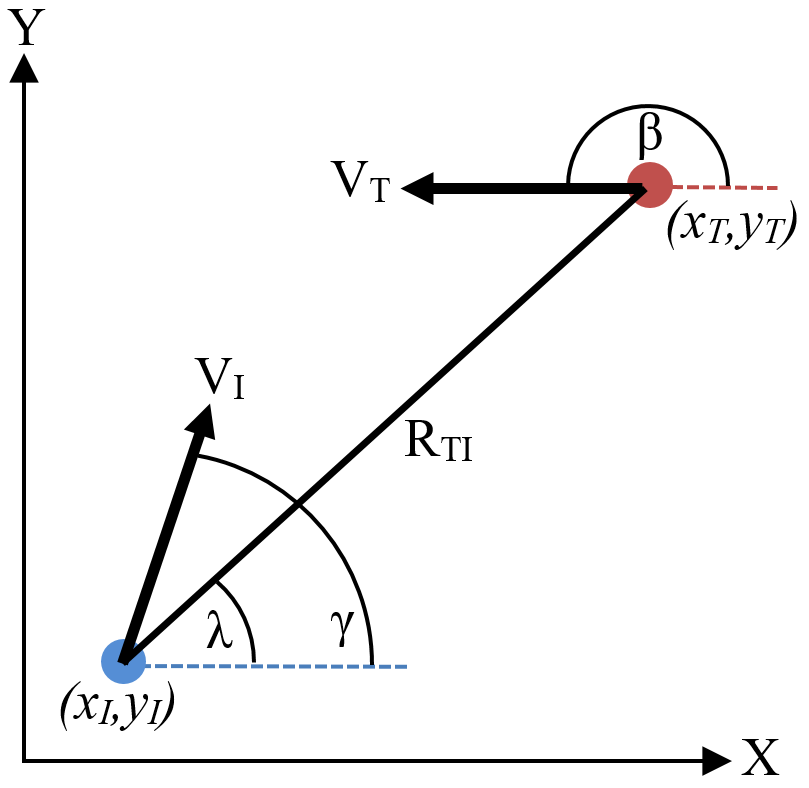
\includegraphics[width=6 cm]{Engagement_Model.PNG}
	\caption{\DIFdelbeginFL %DIFDELCMD < \hl{Interceptor and Target Engagement Scenario (x-East, y-Up)}%%%
\DIFdelendFL \DIFaddbeginFL \DIFaddFL{Engagement Scenario}\DIFaddendFL }
	\label{fig:Egagement}
\end{figure}

The \DIFdelbegin \DIFdel{PN guidance law operates }\DIFdelend \DIFaddbegin \DIFadd{interceptor is guided to the target's position by updating the interceptors heading at each time step $k$. Heading changes are determined by the PN guidance algorithm operating }\DIFaddend on the principle of \DIFdelbegin \DIFdel{modifying heading so that the line-of-sight rate (LOS ) }\DIFdelend \DIFaddbegin \DIFadd{nulling the LOS rate }\DIFaddend $\dot{\lambda}$ \DIFdelbegin \DIFdel{is null. The input rate $\dot{u}$ is }\DIFdelend \DIFaddbegin \DIFadd{by issuing heading change commands }\DIFaddend proportional to the LOS rate\DIFdelbegin \DIFdel{and a }\DIFdelend \DIFaddbegin \DIFadd{. For a non zero LOS rate, a heading rate command $\dot{\gamma}$ is issued by multiplying the LOS rate by the }\DIFaddend fixed guidance gain $N$.
\DIFdelbegin \DIFdel{Second order Runge-Kutta integration was used to determine $u$ from Equation \ref{eq:PNlaw}.
}\DIFdelend 

\begin{equation} \label{eq:PNlaw}
\DIFdelbegin %DIFDELCMD < \dot{u} %%%
\DIFdelend \DIFaddbegin \dot{\gamma} \DIFaddend = N\dot{\lambda}
\end{equation}

Guidance gains of $N < 3$ are generally referred to as conservative while $N > 5$ are referred to as more aggressive\DIFdelbegin \DIFdel{\mbox{%DIFAUXCMD
\cite{zarchan}}\hspace{0pt}%DIFAUXCMD
}\DIFdelend . Conservative gains \DIFdelbegin \DIFdel{result in }\DIFdelend \DIFaddbegin \DIFadd{lead to }\DIFaddend larger turn radii \DIFdelbegin \DIFdel{whereas larger }\DIFdelend \DIFaddbegin \DIFadd{and make for a less maneuverable interceptor. Higher }\DIFaddend gains result in \DIFdelbegin \DIFdel{smaller turn radii. }%DIFDELCMD < \hl{Multi-rotors are capable of making abrupt heading changes in comparison to fixed wing UAVs and it was assumed a guidance gain of $N = 5$ is not beyond multi-rotor capability. The resulting guidance is expected to return sharp turns and straight line optimal paths when used with the Dubins kinematic model.} %%%
\DIFdel{The LOS angle and rate are calculated in Equations \ref{eq:LOS} and \ref{eq:losrate} }\DIFdelend \DIFaddbegin \DIFadd{a more maneuverable vehicle as long as the commanded heading changes are not beyond the vehicles physical capabilities. Multi-rotor UAVs are agile and can make abrupt heading changes therefore a guidance gain $N = 5$ was chosen. The LOS rate is provided by Equation \ref{eq:losrate}, which requires the relative position and velocity components $R_{TIx}$,$R_{TIy}$, and $V_{TIx}$, $V_{TIy}$ shown in Equations \ref{eq:pos} and \ref{eq:vel} }\DIFaddend respectively. 

%DIF < \begin{equation} \label{eq:losrate}
%DIF < \dot{\lambda} = \frac{R_{TIx}V_{TIy}-R_{TIy}V_{TIx}}{R_{TI}^2}
%DIF < \end{equation}
\DIFaddbegin \begin{equation} \DIFadd{\label{eq:losrate}
\dot{\lambda} = \frac{R_{TIx}V_{TIy}-R_{TIy}V_{TIx}}{R_{TI}^2}
}\end{equation}
\DIFaddend 

\begin{equation} \DIFdelbegin %DIFDELCMD < \label{eq:LOS}
%DIFDELCMD < %%%
\DIFdel{\lambda = \tan^{-1} }%DIFDELCMD < \left(%%%
\DIFdel{\frac{y_T - y_I}{x_T - x_I}}%DIFDELCMD < \right)
%DIFDELCMD < %%%
\DIFdelend \DIFaddbegin \label{eq:pos}
\begin{split}
R_{TIx} = x_T-x_I\\
R_{TIy} = y_T-y_I
\end{split}
\DIFaddend \end{equation}

\DIFdelbegin \begin{displaymath} \DIFdel{%DIFDELCMD < \label{eq:losrate}%%%
\dot{\lambda} = \frac{(x_T - x_I)(V_{Ty}-V_{Iy}) - (y_T - y_I)(V_{Tx}-V_{Ix})}{(x_T - x_I)^2+(y_T - y_I)^2}
}\end{displaymath}
%DIFAUXCMD
\DIFdelend \DIFaddbegin \begin{align}
\DIFadd{\label{eq:vel}
\begin{split}
V_{TIx} &= V_{Tx}-V_{Ix}
\\
V_{TIy} &= V_{Ty}-V_{Iy}
\\
\end{split}
}\end{align}
\DIFaddend 

%DIF < \begin{equation} \label{eq:pos}
%DIF < \begin{split}
%DIF < R_{TIx} = x_T-x_I\\
%DIF < R_{TIy} = y_T-y_I
%DIF < \end{split}
%DIF < \end{equation}
%DIF < 
%DIF < \begin{align}
%DIF < \label{eq:vel}
%DIF < \begin{split}
%DIF < V_{TIx} &= V_{Tx}-V_{Ix}
%DIF < \\
%DIF < V_{TIy} &= V_{Ty}-V_{Iy}
%DIF < \\
%DIF < \end{split}
%DIF < \end{align}
\DIFdelbegin %DIFDELCMD < 

%DIFDELCMD < %%%
\DIFdelend Range is the Euclidean distance between the target and the interceptor, shown in Equation \ref{eq:range}. \DIFaddbegin \DIFadd{The LOS angle $\lambda$ is calculated in Equation \ref{eq:LOS}. 
}\DIFaddend 

\begin{equation} \label{eq:range}
R_{TI} =\sqrt[]{\DIFdelbegin \DIFdel{(x_T - x_I)}\DIFdelend \DIFaddbegin \DIFadd{R_{TIx}}\DIFaddend ^2+\DIFdelbegin \DIFdel{((y_T - y_I)}\DIFdelend \DIFaddbegin \DIFadd{R_{TIy}}\DIFaddend ^2}
\end{equation}

%DIF < The PN guidance law provides a heading rate whereas the model requires a heading. To determine the heading from the heading rate, the second order Runge-Kutta integration technique was used. 
\DIFaddbegin \begin{equation} \DIFadd{\label{eq:LOS}
\lambda = \tan^{-1} \left(\frac{R_{TIy}}{R_{TIx}}\right)
}\end{equation}
\DIFaddend 

%DIF < \begin{equation} \label{gamma}
%DIF < \frac{d\gamma}{dt} = \dot{\gamma}
%DIF < \end{equation}
\DIFaddbegin \DIFadd{The PN guidance law provides a heading rate whereas the model requires a heading. To determine the heading from the heading rate, the second order Runge-Kutta integration technique is used. 
}\DIFaddend 

\DIFaddbegin \begin{equation} \DIFadd{\label{gamma}
\frac{d\gamma}{dt} = \dot{\gamma}
}\end{equation}

\DIFaddend % Now consider the same engagement scenario where an interceptor is tasked with intercepting a target except now the exact position of the target is unknown. The intercepting UAV uses on-board sensors to take measurements of the targets position, where each measurement has some uncertainty associated with it. The measurement can be represented as a point centered in a circle of radius $r$. \hl{The radius $r$ represents the domain where the interceptor can be certain that the target exists given the measurement within $n$ standard deviations.} The goal of the interceptor is not to only intercept the target, but to follow it to gather more information. In order to follow the target, it is important to insure that there is not an in-air collision prior to the appropriate time. To prevent an unintended collision, a modified version of the PN guidance is presented. 

% Figure \ref{fig:pseudotarget} depicts a modified engagement strategy involving a target and an interceptor. The exact position of the intercepting UAV is unknown, however the position of the target with some uncertainty $r$ is estimated. The intercepting UAV is tasked with intercepting and following the target, but is given the restriction that it cannot enter the airspace where the target may actually be. To safely intercept and follow the target, the intercepting UAV will follow the process depicted in Figure \ref{fig:pseudotarget}. \\

% The interceptor is tasked with following a pseudo-target that is placed strategically to promote target interception and following while preventing an in air collision of the vehicles. The pseudo-target is first placed at $(0,0)$ and remains in place until the minimum point on the uncertainty bubble is above the horizon. Once the minimum point of the uncertainty bubble is above the horizon, the pseudo-target is placed at $(0, r_{ymin})$ as shown in \ref{fig:pseudotarget}a. The interceptor follows the pseudo-target placed at the minimum point of the uncertainty bubble present at $x = 0$ in \ref{fig:pseudotarget}b and \ref{fig:pseudotarget}c. Once the uncertainty bubble has passed the $y$ plane, the pseudo-target is placed on top of the targets estimated position, forcing the interceptor to enter a follow pattern shown in \ref{fig:pseudotarget}d. 


PN guidance is effective at reducing the range between the interceptor and the target, however \DIFdelbegin \DIFdel{when range is near zero }\DIFdelend \DIFaddbegin \DIFadd{at or near the point of interception }\DIFaddend a singularity in the LOS rate \DIFdelbegin \DIFdel{will occur }\DIFdelend \DIFaddbegin \DIFadd{may be present }\DIFaddend for head-on \DIFdelbegin \DIFdel{intercept, shown in Figure \ref{fig:failedIntercept} and \ref{fig:failedInterceptLOS}. The singularity is caused by a combination of relative velocity sign change and division by zero}\DIFdelend \DIFaddbegin \DIFadd{interception. The cause of the singularity is due to the near zero range and the change of sign in relative velocities}\DIFaddend . Solutions around the singularity can be obtained for a linearized proportional navigation \cite{singularitySolution} but are not \DIFdelbegin \DIFdel{a }\DIFdelend \DIFaddbegin \DIFadd{of a major }\DIFaddend concern for traditional missile systems because the mission is complete when the range is near zero. For an intercepting UAV with the intention of following the target, \DIFdelbegin \DIFdel{a singularity calls }\DIFdelend \DIFaddbegin \DIFadd{the singularity could call }\DIFaddend for control efforts beyond the saturation point. \DIFdelbegin \DIFdel{After }\DIFdelend \DIFaddbegin \DIFadd{Additionally, after }\DIFaddend the singularity occurs there remains a possibility for the nulled LOS condition to be met even if the interceptor and target are heading away from each other. \DIFdelbegin %DIFDELCMD < \hl{Figure} %%%
\DIFdel{\ref{fig:failedIntercept} }%DIFDELCMD < \hl{demonstrates how for head-on intercepts the nulled LOS rate can be satisfied and the interceptor flys away from the target. Figure} %%%
\DIFdel{\ref{fig:failedInterceptLOS} }%DIFDELCMD < \hl{shows how a singularity can occur near zero range.}
%DIFDELCMD < 

%DIFDELCMD < %%%
%DIF <  Demonstrating the effectiveness of the PN guidance algorithm at reducing the range between a target and an interceptor, 
%DIF <  The PN guidance reduces the range between the interceptor and target as shown in Figure \ref{fig:comp}. 
%DIFDELCMD < 

%DIFDELCMD < \begin{figure}[H]
%DIFDELCMD < 	\centering
%DIFDELCMD < 	\includegraphics[width=7cm] {%%%
\DIFdelFL{failedHeadOn}%DIFDELCMD < }
%DIFDELCMD < 	%%%
%DIFDELCMD < \caption{%
{%DIFAUXCMD
\DIFdelFL{Failed follow for head on intercept}}
	%DIFAUXCMD
%DIFDELCMD < \label{fig:failedIntercept}
%DIFDELCMD < 	%%%
\DIFdelFL{\hspace*{0mm}
}%DIFDELCMD < \end{figure}
%DIFDELCMD < 

%DIFDELCMD < \begin{figure}[H]
%DIFDELCMD < 	\centering
%DIFDELCMD < 	\includegraphics[width=7cm] {%%%
\DIFdelFL{x50_range_LOSrate}%DIFDELCMD < }
%DIFDELCMD < 	%%%
%DIFDELCMD < \caption{%
{%DIFAUXCMD
\DIFdelFL{Failed follow with LOS-rate singularity and range}}
	%DIFAUXCMD
%DIFDELCMD < \label{fig:failedInterceptLOS}
%DIFDELCMD < 	%%%
\DIFdelFL{\hspace*{0mm}
}%DIFDELCMD < \end{figure}
%DIFDELCMD < 

%DIFDELCMD < %%%
\DIFdel{The interceptor does not fail to intercept and follow the target for a }\DIFdelend \DIFaddbegin \DIFadd{For an inbound target with a 1:1 speed ratio constraint, the singularity is not present during a }\DIFaddend tail-chase \DIFdelbegin \DIFdel{scenario }\DIFdelend \DIFaddbegin \DIFadd{intercept as }\DIFaddend shown in Figure \DIFdelbegin \DIFdel{\ref{fig:successfulFollow} and no singularities are present in Figure \ref{fig:successfulFollowLOS}}\DIFdelend \DIFaddbegin \DIFadd{\ref{fig:comp}}\DIFaddend . The tail-chase scenario has the added benefit of placing the interceptor behind the target, allowing for \DIFdelbegin \DIFdel{a }\DIFdelend \DIFaddbegin \DIFadd{an easy }\DIFaddend transition into a follow. The elimination of the singularity and easy transition into a follow make a case for waiting on the target before intercepting it directly, which is the \DIFaddbegin \DIFadd{primary }\DIFaddend motivation for introducing a pseudotarget into the PN guidance model.




%DIF >  Demonstrating the effectiveness of the PN guidance algorithm at reducing the range between a target and an interceptor, 
%DIF >  The PN guidance reduces the range between the interceptor and target as shown in Figure \ref{fig:comp}. 
\DIFaddbegin 

\DIFaddend \begin{figure}[H]
	\DIFaddbeginFL \begin{subfigmatrix}{2}%DIF >  number of columns
		\DIFaddendFL \centering
		\DIFaddbeginFL \subfigure []{\DIFaddendFL \includegraphics[width=7cm] {\DIFdelbeginFL \DIFdelFL{tailChaseWithLedgend}\DIFdelendFL \DIFaddbeginFL \DIFaddFL{x50}\DIFaddendFL }\DIFdelbeginFL %DIFDELCMD < \caption{%
{%DIFAUXCMD
\DIFdelFL{Successful follow for tail chase intercept}}
	%DIFAUXCMD
%DIFDELCMD < \label{fig:successfulFollow}
%DIFDELCMD < 	%%%
\DIFdelFL{\hspace*{0mm}
}%DIFDELCMD < \end{figure}
%DIFDELCMD < 

%DIFDELCMD < \begin{figure}[H]
%DIFDELCMD < 	\centering
%DIFDELCMD < 	%%%
\DIFdelendFL \DIFaddbeginFL }
		\subfigure []{\DIFaddendFL \includegraphics[width=7cm] {x15\DIFaddbeginFL }}
		\subfigure []{\includegraphics [\DIFaddFL{width=7cm}]{\DIFaddFL{x50}\DIFaddendFL _range_LOSrate}\DIFdelbeginFL %DIFDELCMD < \caption{%
{%DIFAUXCMD
\DIFdelFL{Successful follow LOS-rate and range}}
	%DIFAUXCMD
%DIFDELCMD < \label{fig:successfulFollowLOS}
%DIFDELCMD < 		%%%
\DIFdelFL{\hspace*{0mm}
	}\DIFdelendFL \DIFaddbeginFL }
		\subfigure []{\includegraphics [\DIFaddFL{width=7cm}]{\DIFaddFL{x15_range_LOSrate}}}
		\DIFaddFL{\hspace*{0mm}
	}\end{subfigmatrix}
	\caption{\DIFaddFL{Simulation Scenarios}}
	\label{fig:comp}
\DIFaddendFL \end{figure}


%DIF < \begin{figure}[h]
%DIF < 	\begin{subfigmatrix}{1}% number of columns
%DIF < 		\centering
%DIF < 		\subfigure []{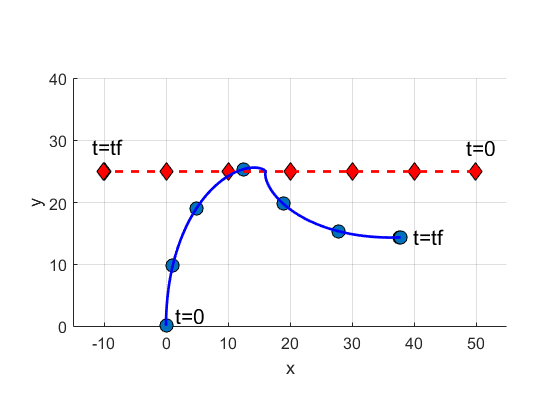
\includegraphics[width=7cm] {x50}}
%DIF < 		\subfigure []{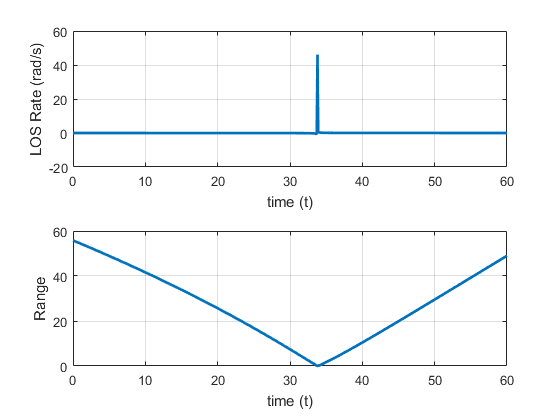
\includegraphics [width=7cm]{x50_range_LOSrate}}
%DIF < %		\caption{Failed}
%DIF < %		\subfigure []{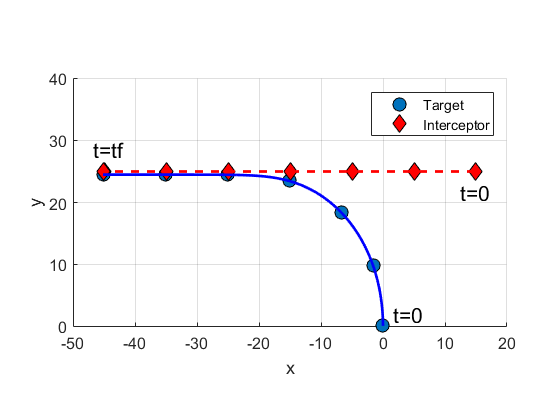
\includegraphics[width=7cm] {x15}}
%DIF < %	
%DIF < %		\subfigure []{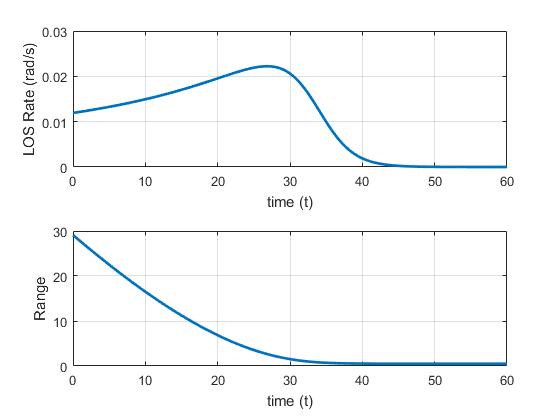
\includegraphics [width=7cm]{x15_range_LOSrate}}
%DIF < 		\hspace*{0mm}
%DIF < 	\end{subfigmatrix}
%DIF < 	\caption{Simulation Scenarios}
%DIF < 	\label{fig:comp}
%DIF < \end{figure}
\DIFdelbegin %DIFDELCMD < 

%DIFDELCMD < %%%
%DIF < \begin{figure}[h]
%DIF < 	\begin{subfigmatrix}{1}% number of columns
%DIF < 		\centering
%DIF < %		\subfigure []{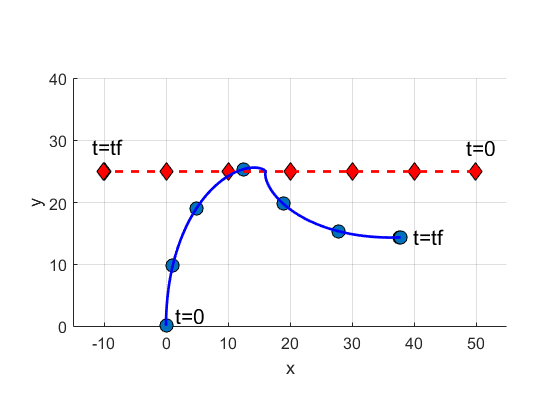
\includegraphics[width=7cm] {x50}}
%DIF < %		\subfigure []{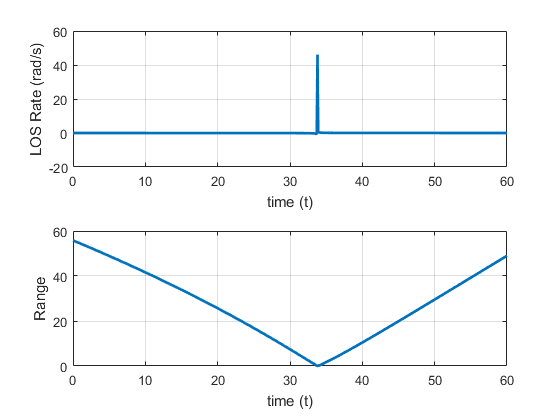
\includegraphics [width=7cm]{x50_range_LOSrate}}
%DIF < %		%		\caption{Failed}
%DIF < 		\subfigure []{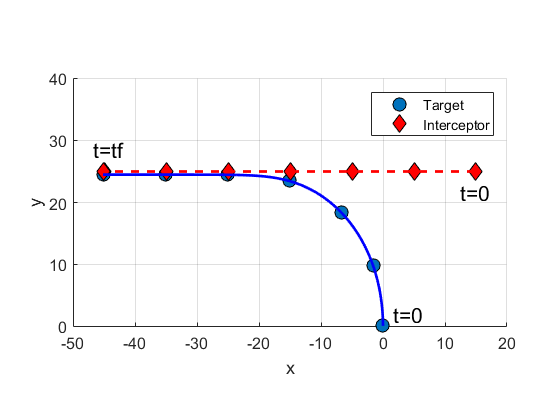
\includegraphics[width=7cm] {x15}}
%DIF < 		
%DIF < 		\subfigure []{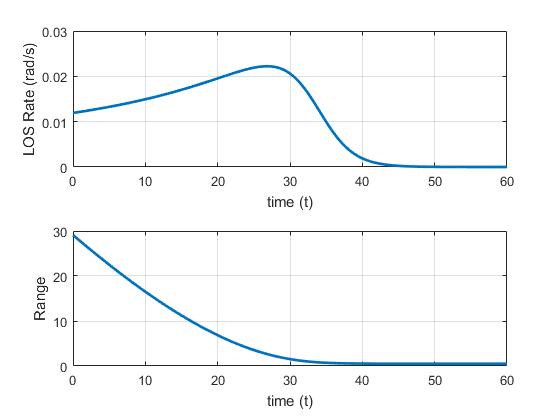
\includegraphics [width=7cm]{x15_range_LOSrate}}
%DIF < 		\hspace*{0mm}
%DIF < 	\end{subfigmatrix}
%DIF < 	\caption{Simulation Scenarios}
%DIF < 	\label{fig:comp}
%DIF < \end{figure}
%DIFDELCMD < 

%DIFDELCMD < %%%
\DIFdelend \subsection{Intercept and Follow Model}
Measuring the LOS rate and range \DIFdelbegin \DIFdel{uncertainties }\DIFdelend \DIFaddbegin \DIFadd{would be done by on-board sensors which would have some uncertainty $r$. Uncertainties }\DIFaddend in $x$ and $y$ are assumed to be equal so the actual position of the target is in the space \DIFdelbegin \DIFdel{$(x_T\pm r,y_T \pm r)$, where $r$ is the radius of uncertainty}\DIFdelend \DIFaddbegin \DIFadd{$(x\pm r,y \pm r)$}\DIFaddend . Figure \ref{fig:uncertrad} shows a representation of the measurement as a point centered in a circle of radius $r$. The region inside the circle is the space where the target may actually exist. The interceptor should avoid the inside of the circular region to prevent an unintended collision with the target. The uncertainty decreases linearly as a function of range as shown in Equations \ref{eq:uncert} and \ref{beq}.

\begin{figure}[H]
	\centering
	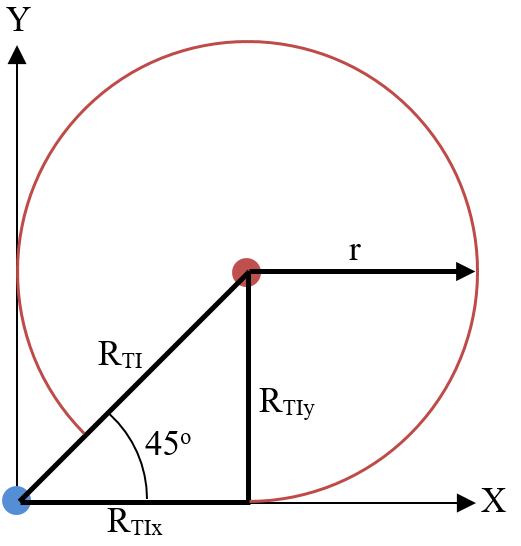
\includegraphics[width=4cm]{45deguncert.PNG}
	\caption{\DIFdelbeginFL \DIFdelFL{Position uncertainty radius centered on target}\DIFdelendFL \DIFaddbeginFL \DIFaddFL{Initial Uncertainty Radius}\DIFaddendFL }
	\label{fig:uncertrad}
\end{figure}

%DIF < \begin{equation} \label{eq:uncert}
%DIF < r(k) = drR_{TI}+b
%DIF < \end{equation}
\DIFaddbegin \begin{equation} \DIFadd{\label{eq:uncert}
r(k) = drR_{TI}(k)+b
}\end{equation}
\DIFaddend 

\begin{equation} \DIFdelbegin %DIFDELCMD < \label{eq:uncert}
%DIFDELCMD < %%%
\DIFdel{r = dr \,\sqrt[}%DIFDELCMD < ]{%%%
\DIFdel{(x_T - x_I)^2+(y_T - y_I)^2}%DIFDELCMD < }%%%
\DIFdel{+}\DIFdelend \DIFaddbegin \label{beq}
\DIFaddend b \DIFaddbegin \DIFadd{= r_0-drR_{TI0}
}\DIFaddend \end{equation}

%DIF < \begin{equation} \label{beq}
%DIF < b = r_0-drR_{TI0}
%DIF < \end{equation}
\DIFdelbegin %DIFDELCMD < 

%DIFDELCMD < %%%
\begin{displaymath} \DIFdel{%DIFDELCMD < \label{beq}%%%
b = r_0-dr \,\sqrt[}]{\DIFdel{(x_{T0} - x_{I0})^2+(y_{T0} - y_{I0})^2}}
\end{displaymath}
%DIFAUXCMD
%DIFDELCMD < 

%DIFDELCMD < %%%
\DIFdelend The radius of position uncertainty $r$ \DIFdelbegin \DIFdel{was represented as }\DIFdelend \DIFaddbegin \DIFadd{is }\DIFaddend a function of the range $R_{TI}$, rate of change $dr$, and the minimum uncertainty radius $b$. A pseudotarget was introduced into the engagement scenario which prevents the interceptor from entering the region of uncertainty while maintaining the requirements of intercepting and following the target. The modified guidance was developed to satisfy a small range of scenarios where the target travels at constant heading, altitude, and speed equal to that of the interceptor \DIFaddbegin \DIFadd{shown in Figure \ref{fig:pseudotarget}}\DIFaddend . The interceptor avoids the region of uncertainty while following and intercepting the target by pursuing a pseudotarget. 

The pseudotarget \DIFdelbegin \DIFdel{acted }\DIFdelend \DIFaddbegin \DIFadd{acts }\DIFaddend as a state machine consisting of $wait$, $intercept$, and $follow$ states\DIFdelbegin \DIFdel{shown in Figures \ref{fig:wait}, \ref{fig:intercept}, and \ref{fig:follow} respectively}\DIFdelend . When the minimum altitude of the uncertainty is below the horizon $y_I-r<0$ the pseudotarget \DIFdelbegin %DIFDELCMD < \hl{'s} %%%
\DIFdelend state is set to \DIFdelbegin %DIFDELCMD < \hl{$wait$} %%%
\DIFdelend \DIFaddbegin \DIFadd{$wat$ }\DIFaddend and waits at it's current position. Uncertainty decreases as the target approaches the interceptor eventually satisfying the condition $y_I-r >0$ triggering a change in state from \DIFdelbegin \DIFdel{$wait$ }\DIFdelend \DIFaddbegin \DIFadd{$wiat$ }\DIFaddend to $intercept$. When the $intercept$ state is active the pseudotarget is placed at the minimum uncertainty $y=y_T-r$ with no movement in the $x$ axis \DIFdelbegin \DIFdel{, }\DIFdelend $x=0$. Placing the pseudotarget at the minimum uncertainty altitude prevents the possibility of an unintended collision with the target. \DIFdelbegin %DIFDELCMD < \hl{Intercept is intended to reduce the range to the target and get close, but not result in a collision. Once $x_T<x_I$ the problem becomes a tail chase scenario and the risk of collision is non existent.} %%%
\DIFdel{The algorithm is }\DIFdelend \DIFaddbegin \DIFadd{Once $x_T<x_I$ the risk of collision is non existent and the pseudotarget is }\DIFaddend set to the $follow$ state where the pseudotarget is placed on top of the targets estimated position. \DIFaddbegin \DIFadd{The engagement described is shown in \ref{fig:pseudotarget}.
}\DIFaddend 

% is placed at $x = 0$ and $y = y_T-r$. 

% Placing the pseudotarget at the edge of the uncertainty region prevents the possibility of an unintended collision. 


% a the pseudotarget $waits$ while the minimum uncertainty is below the horizon.

% When in $intercept$ state, the pseudotarget guides the intercepting UAV to the target, closing the distance between the two. During the $follow$ state, the pseudotarget guides the interceptor to follow the target.

% When in $intercept$ state, the pseudotarget is placed at the minimum altitude of the uncertainty region that is to the right of the interceptor. During $follow$, the pseudotarget is placed directly on top of the target's estimated position.

\begin{figure}[H]
	\DIFaddbeginFL \begin{subfigmatrix}{3}%DIF >  number of columns
		\DIFaddendFL \centering
		\DIFdelbeginFL %DIFDELCMD < 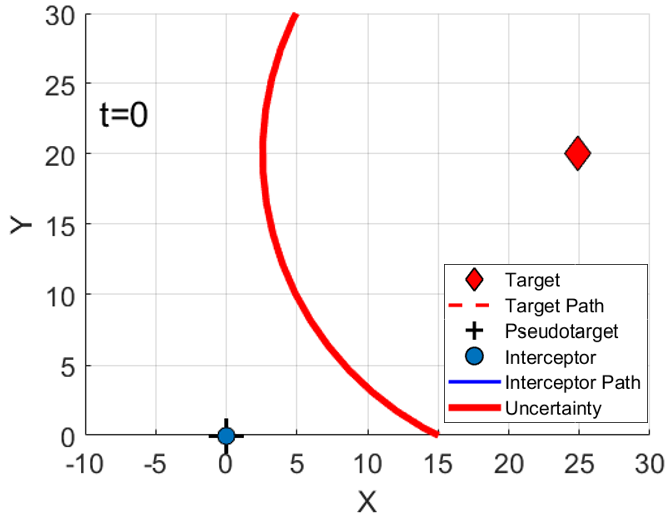
\includegraphics[width=7cm]{wait}
%DIFDELCMD < 	%%%
\DIFdelendFL \DIFaddbeginFL \subfigure []{\includegraphics[width=5cm] {\DIFaddFL{step1}}}
		\subfigure []{\includegraphics[width=5cm] {\DIFaddFL{step2}}}
		\subfigure []{\includegraphics [\DIFaddFL{width=5cm}]{\DIFaddFL{step3}}}
	\end{subfigmatrix}
	\DIFaddendFL \caption{\DIFdelbeginFL \DIFdelFL{Uncertainty below the horizon sets pseudotarget state to wait}\DIFdelendFL \DIFaddbeginFL \DIFaddFL{Simulation Scenarios}\DIFaddendFL }
	\DIFdelbeginFL %DIFDELCMD < \label{fig:wait}
%DIFDELCMD < %%%
\DIFdelendFL \DIFaddbeginFL \label{fig:pseudotarget}
\DIFaddendFL \end{figure}

\DIFdelbegin %DIFDELCMD < \begin{figure}[H]
%DIFDELCMD < 	\centering
%DIFDELCMD < 	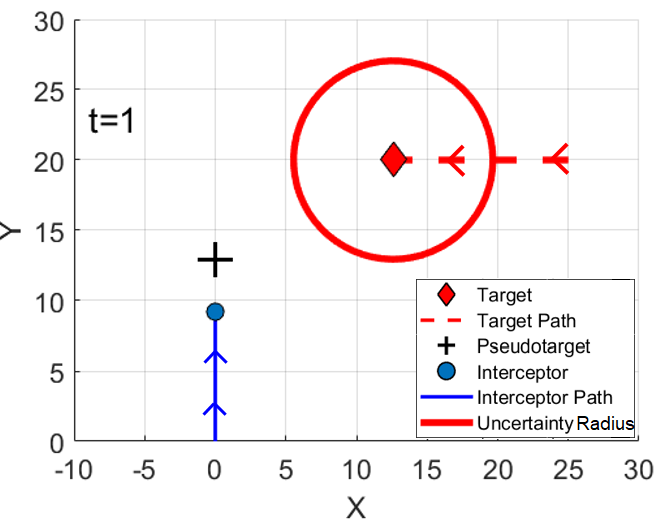
\includegraphics[width=7cm]{intercept}
%DIFDELCMD < 	%%%
%DIFDELCMD < \caption{%
{%DIFAUXCMD
\DIFdelFL{Uncertainty above the horizon sets pseudotarget state to intercept}}
	%DIFAUXCMD
%DIFDELCMD < \label{fig:intercept}
%DIFDELCMD < \end{figure}
%DIFDELCMD < 

%DIFDELCMD < \begin{figure}[H]
%DIFDELCMD < 	\centering
%DIFDELCMD < 	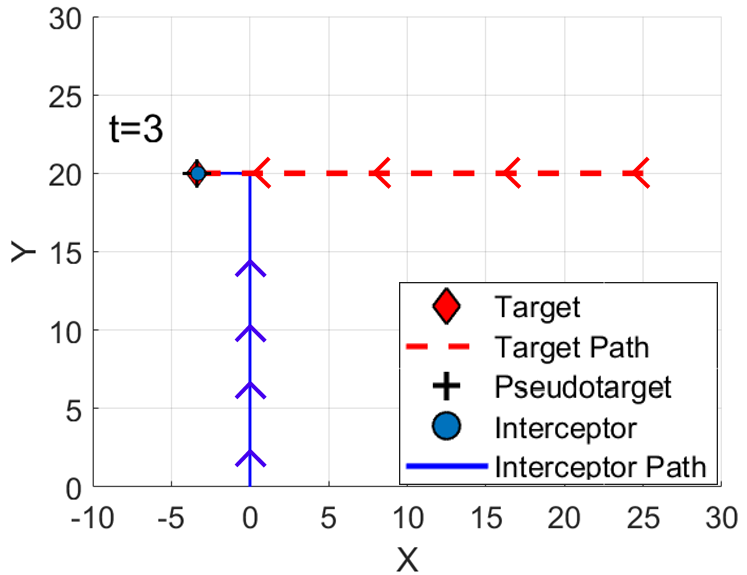
\includegraphics[width=7cm]{follow}
%DIFDELCMD < 	%%%
%DIFDELCMD < \caption{%
{%DIFAUXCMD
\DIFdelFL{Target estimate $x_T < 0$ sets pseudotarget state to follow}}
	%DIFAUXCMD
%DIFDELCMD < \label{fig:follow}
%DIFDELCMD < \end{figure}
%DIFDELCMD < 

%DIFDELCMD < %%%
%DIF < \begin{figure}[H]
%DIF < 	\begin{subfigmatrix}{3}% number of columns
%DIF < 		\centering
%DIF < 		\subfigure []{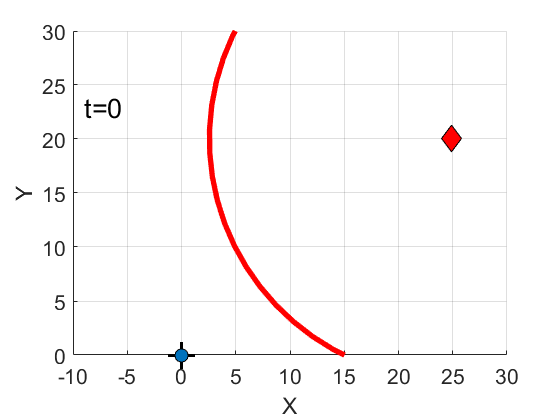
\includegraphics[width=5cm] {step1}}
%DIF < 		\subfigure []{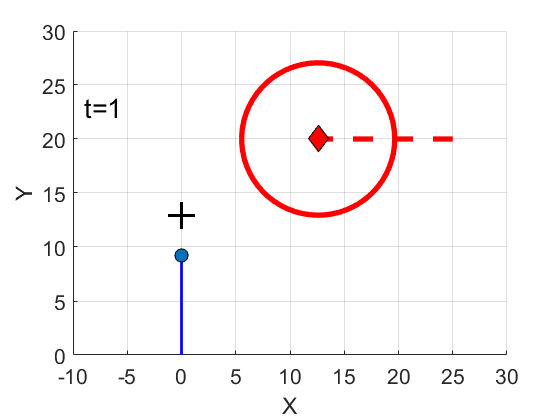
\includegraphics[width=5cm] {step2}}
%DIF < 		\subfigure []{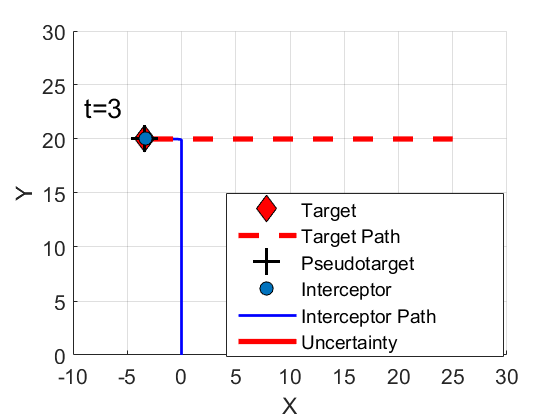
\includegraphics [width=5cm]{step3}}
%DIF < 	\end{subfigmatrix}
%DIF < 	\caption{Simulation Scenarios}
%DIF < 	\label{fig:pseudotarget}
%DIF < \end{figure}
%DIFDELCMD < 

%DIFDELCMD < %%%
\DIFdelend %Change figures to better represent algorithm.
% In Figure \ref{fig:pseudotarget}a the pseudotarget $waits$ while the minimum uncertainty is below the horizon. As the target approaches, the uncertainty is reduced so that the uncertainty circle is above the horizon shown in Figure \ref{fig:pseudotarget}b. With the minimum of the uncertainty above the horizon, the pseudotarget is placed in the $intercept$ state and is placed at $x = 0$ and $y = y_T-r$. Placing the pseudotarget at the edge of the uncertainty region prevents the possibility of an unintended collision. Once $x_T<x_I$ the risk of collision is non existent and the pseudotarget is placed in $follow$ state. The $follow$ state shown in Figure \ref{fig:pseudotarget}c places the pseudotarget on top of the target estimate, guiding the interceptor to follow the target. 

With the target moving at constant altitude and both vehicles sharing the same velocity, it is expected that the following distance will be near zero if the intercept is active when $x_T \geq y_T$. If the intercept occurs when $x_T<y_T$, the interceptor is at a disadvantage and will fail to close the distance. The sensor was modeled so that the uncertainty circle is above the horizon once the target has crossed the $x=y$ line by calculating an appropriate initial uncertainty $r_0$. Referring back to Figure \ref{fig:uncertrad} a target \DIFaddbegin \DIFadd{is detected }\DIFaddend at a LOS of $45^{\circ}$, has an altitude of $R_{TIy}$, and an initial uncertainty radius $r_0$. Determining the initial radius was done geometrically in Equations \ref{minr} and \ref{rtiforminr} and was set to $0.7$ times the initial range.

%DIF < \sqrt[]{(x_T - x_I)^2+(y_T - y_I)^2}
\DIFaddbegin \begin{equation} \DIFadd{\label{minr}
\sin(45) = \frac{R_{TIy}}{R_{TI}}
}\end{equation}
\DIFaddend 

%DIF < \begin{equation} \label{minr}
%DIF < \sin(45^\circ) = \frac{R_{TIy}}{R_{TI}}
%DIF < \end{equation}
\DIFaddbegin \begin{equation} \DIFadd{\label{rtiforminr}
R_{TI}\frac{\sqrt[]{2}}{2} = R_{TIy}
}\end{equation}
\DIFaddend 

\DIFdelbegin \begin{displaymath} \DIFdel{%DIFDELCMD < \label{minr}%%%
\sin(45^\circ) = \frac{y_T - y_I}{\sqrt[]{(x_T - x_I)^2+(y_T - y_I)^2}}
}\end{displaymath}
%DIFAUXCMD
%DIFDELCMD < 

%DIFDELCMD < %%%
\begin{displaymath} \DIFdel{%DIFDELCMD < \label{rtiforminr}%%%
 (y_T - y_I) = \sqrt[}]{\DIFdel{(x_T - x_I)^2+(y_T - y_I)^2}}\DIFdel{\sin(45^\circ)
}\end{displaymath}
%DIFAUXCMD
%DIFDELCMD < 

%DIFDELCMD < %%%
%DIF < \begin{equation} \label{rtiforminr}
%DIF < R_{TI}\frac{\sqrt[]{2}}{2} = R_{TIy}
%DIF < \end{equation}
%DIFDELCMD < 

%DIFDELCMD < %%%
\DIFdelend \begin{equation} \label{initialr}
r_0 = 0.7R_{TI}
\end{equation}

The impact of $r_0$ on following distance can be seen in \DIFdelbegin \DIFdel{Figures \ref{fig:rti07} and \ref{fig:rti08}. Each Figure shows }\DIFdelend \DIFaddbegin \DIFadd{Figure \ref{fig:RinitSelection}, where three $r_0$ ratios were evaluated. Each subfigure show }\DIFaddend the results of three target initial conditions along the $x=y$ line. Figure \DIFdelbegin \DIFdel{\ref{fig:rti07} }\DIFdelend \DIFaddbegin \DIFadd{\ref{fig:RinitSelection}a }\DIFaddend shows a near zero following distance for a $r_0$ ratio of \DIFaddbegin \DIFadd{$0.6R_{TI}$. Figure \ref{fig:RinitSelection}b shows a near zero following distance for a $r_0$ ratio of }\DIFaddend $0.7R_{TI}$. \DIFdelbegin \DIFdel{When $r_0>0.7R_{TI}$ the }\DIFdelend \DIFaddbegin \DIFadd{As the $r_0$ ratio passes $0.7R_{TI}$ the }\DIFaddend following distance becomes less predictable and is not constant along the target initial conditions on the $x=y$ line\DIFdelbegin \DIFdel{as shown in Figure \ref{fig:rti08}}\DIFdelend .


\begin{figure}[H]
	\DIFaddbeginFL \begin{subfigmatrix}{2}%DIF >  number of columns
		\DIFaddendFL \centering
		\DIFdelbeginFL %DIFDELCMD < 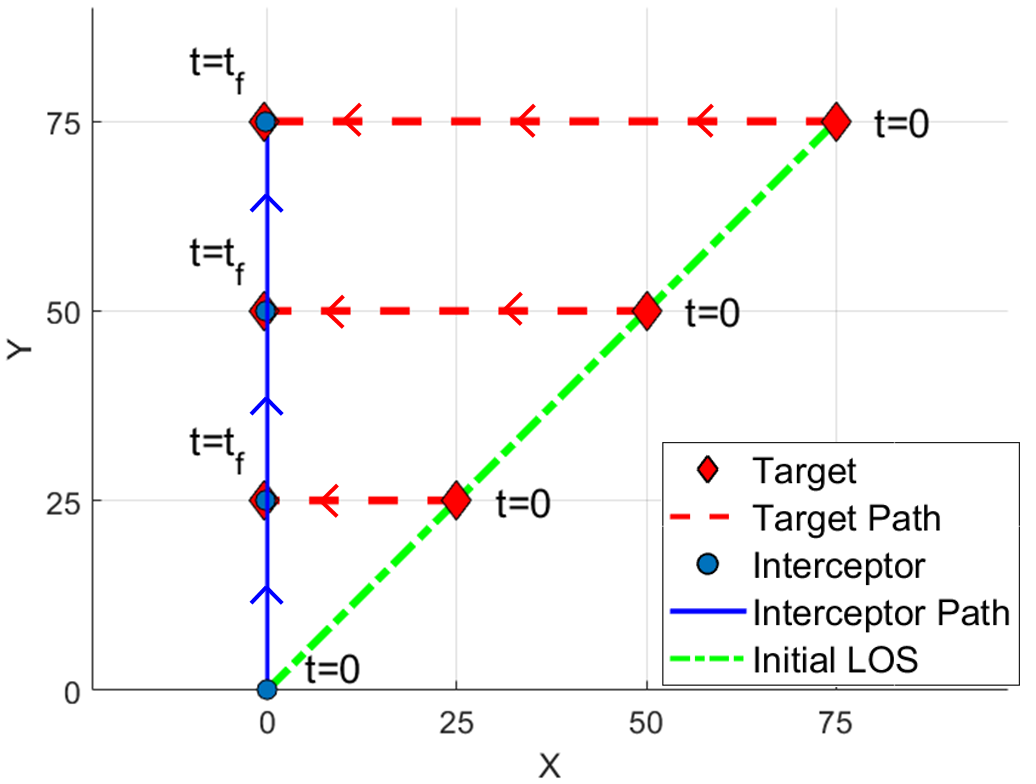
\includegraphics[width=7cm]{Rinit07new.png}
%DIFDELCMD < 	%%%
\DIFdelendFL \DIFaddbeginFL \subfigure []{\includegraphics {\DIFaddFL{rinit07.png}}}
		\subfigure []{\includegraphics {\DIFaddFL{rinit08.png}}}
		\DIFaddFL{\hspace*{0mm}
	}\end{subfigmatrix}
	\DIFaddendFL \caption{Initial \DIFdelbeginFL \DIFdelFL{uncertainty ratio $0.7R_{TI}$ results in consistent following distance}\DIFdelendFL \DIFaddbeginFL \DIFaddFL{Uncertainty Radius Ratio}\DIFaddendFL }
	\DIFdelbeginFL %DIFDELCMD < \label{fig:rti07}
%DIFDELCMD < %%%
\DIFdelendFL \DIFaddbeginFL \label{fig:RinitSelection}
\DIFaddendFL \end{figure}

\DIFdelbegin %DIFDELCMD < \begin{figure}[H]
%DIFDELCMD < 	\centering
%DIFDELCMD < 	\includegraphics[width=7cm]{rinit08new.png}
%DIFDELCMD < 	%%%
%DIFDELCMD < \caption{%
{%DIFAUXCMD
\DIFdelFL{Initial uncertainty ratio $>0.7R_{TI}$ results in increasing following distance as initial range increases}}
	%DIFAUXCMD
%DIFDELCMD < \label{fig:rti08}
%DIFDELCMD < \end{figure}
%DIFDELCMD < 

%DIFDELCMD < %%%
%DIF < \begin{figure}[H]
%DIF < 	\begin{subfigmatrix}{2}% number of columns
%DIF < 		\centering
%DIF < 		\subfigure []{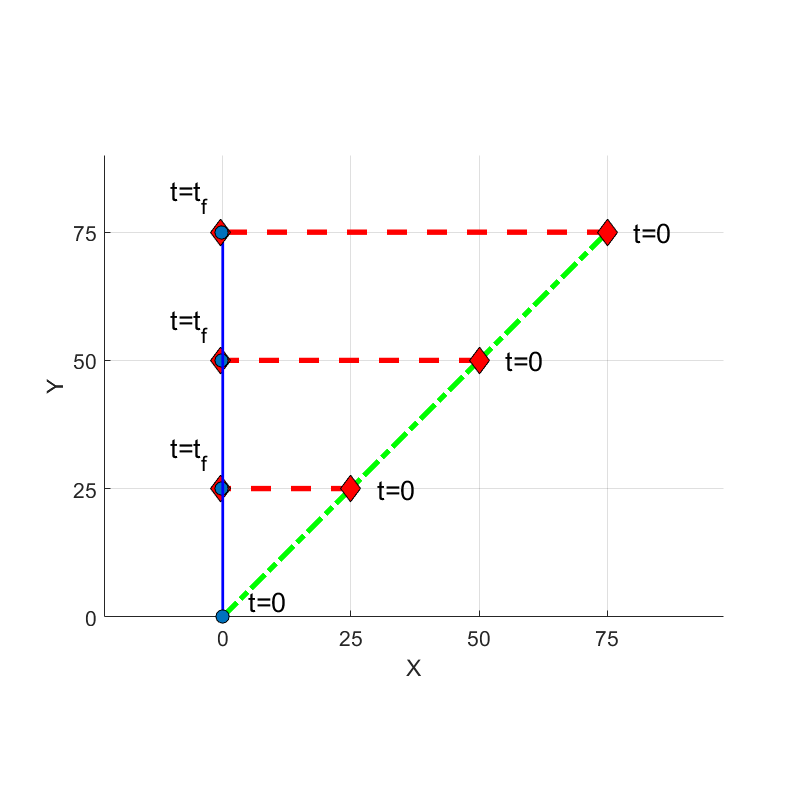
\includegraphics {rinit07.png}}
%DIF < 		\subfigure []{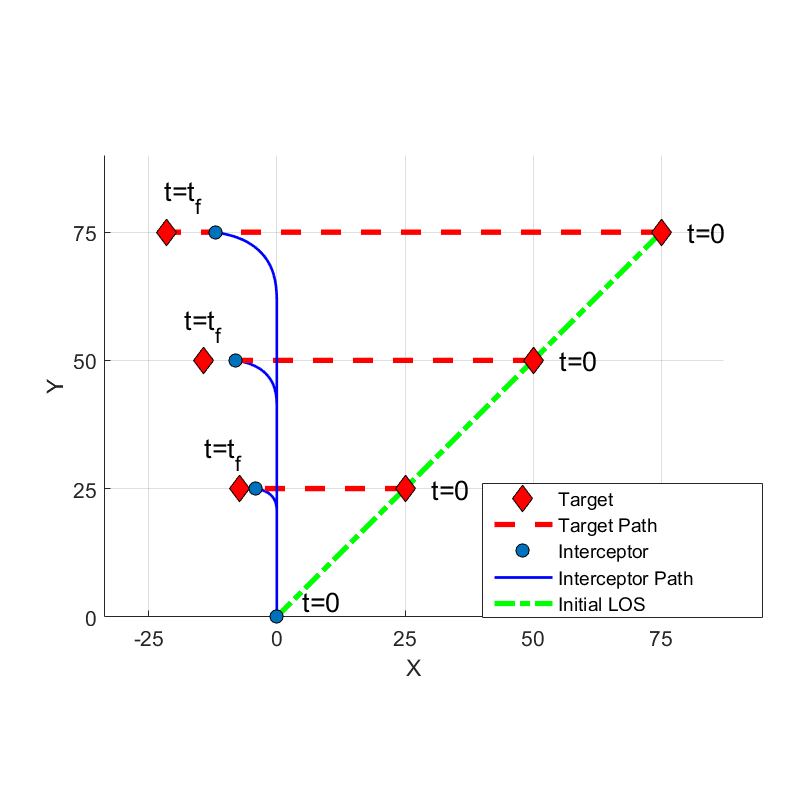
\includegraphics {rinit08.png}}
%DIF < 		\hspace*{0mm}
%DIF < 	\end{subfigmatrix}
%DIF < 	\caption{Initial uncertainty ratio a) $0.7R_{TI}$ results in consistent following distance b)$<0.7R_{TI}$ results in increasing following distance as initial range increases}
%DIF < 	\label{fig:RinitSelection}
%DIF < \end{figure}
%DIFDELCMD < 

%DIFDELCMD < %%%
\DIFdelend The modified pseudotarget PN guidance was given the same initial conditions as shown in Figure \DIFdelbegin \DIFdel{\ref{fig:failedIntercept} }\DIFdelend \DIFaddbegin \DIFadd{\ref{fig:comp} }\DIFaddend and the performance compared. Traditional PN guidance performed well during the tail-chase but failed to follow the target and experienced a LOS singularity for a head-on intercept. The PN guidance with a psuedotarget successfully intercepts and follows the target \DIFdelbegin \DIFdel{, Figure \ref{fig:modifiedPNsuccess}, }\DIFdelend with non-singularity LOS rates, shown in Figure \DIFdelbegin \DIFdel{\ref{fig:modifiedPNsuccessLOS}}\DIFdelend \DIFaddbegin \DIFadd{\ref{fig:compwithpt}}\DIFaddend . Traditional PN out performed the pseudotarget PN guidance for target initial condition $x_{T} = 15$ which demonstrates that a single guidance algorithm may not be suitable for all cases and a decision on which algorithm to use for a given set of initial conditions should be made. Table \ref{my-label} summarizes the performance of the algorithms for the two initial conditions.

\begin{figure}[H]
	\DIFaddbeginFL \begin{subfigmatrix}{2}%DIF >  number of columns
		\DIFaddendFL \centering
		\DIFdelbeginFL %DIFDELCMD < \includegraphics[width=7cm] %%%
\DIFdelendFL \DIFaddbeginFL \subfigure []\DIFaddendFL {\DIFdelbeginFL \DIFdelFL{fixedSingularity}\DIFdelendFL \DIFaddbeginFL \includegraphics[width=4cm] {\DIFaddFL{ptx50}\DIFaddendFL }\DIFdelbeginFL %DIFDELCMD < \caption{%
{%DIFAUXCMD
\DIFdelFL{Tail chase with no singularities, and steady state range $R_{TI}\approx0$}}
	%DIFAUXCMD
%DIFDELCMD < \label{fig:modifiedPNsuccess}
%DIFDELCMD < 	%%%
\DIFdelFL{\hspace*{0mm}
}%DIFDELCMD < \end{figure}
%DIFDELCMD < 

%DIFDELCMD < \begin{figure}[H]
%DIFDELCMD < 	\centering
%DIFDELCMD < 	\includegraphics[width=7cm] %%%
\DIFdelendFL \DIFaddbeginFL }
		\subfigure []\DIFaddendFL {\DIFaddbeginFL \includegraphics[width=4cm] {\DIFaddFL{ptx15}}}
		\subfigure []{\includegraphics [\DIFaddFL{width=4cm}]{\DIFaddendFL ptx50_range_LOSrate}\DIFdelbeginFL %DIFDELCMD < \caption{%
{%DIFAUXCMD
\DIFdelFL{Tail chase with no singularities, and steady state range $R_{TI}\approx0$}}
	%DIFAUXCMD
%DIFDELCMD < \label{fig:modifiedPNsuccessLOS}
%DIFDELCMD < 	%%%
\DIFdelFL{\hspace*{0mm}
	}\DIFdelendFL \DIFaddbeginFL }
		\subfigure []{\includegraphics [\DIFaddFL{width=4cm}]{\DIFaddFL{ptx15_range_LOSrate}}}
		\DIFaddFL{\hspace*{0mm}
	}\end{subfigmatrix}
	\caption{\DIFaddFL{Simulation Scenarios}}
	\label{fig:compwithpt}
\DIFaddendFL \end{figure}

%DIF < \begin{figure}[H]
%DIF < 	\begin{subfigmatrix}{2}% number of columns
%DIF < 		\centering
%DIF < 		\subfigure []{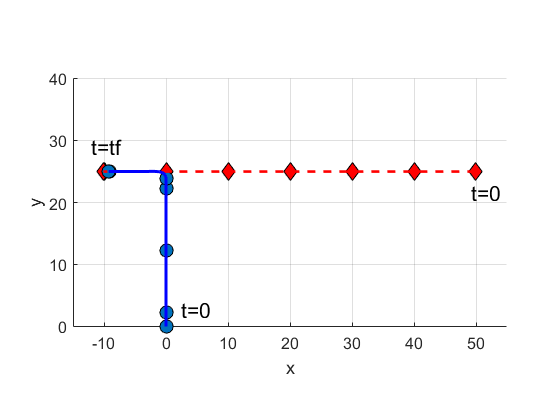
\includegraphics[width=4cm] {ptx50}}
%DIF < 		\subfigure []{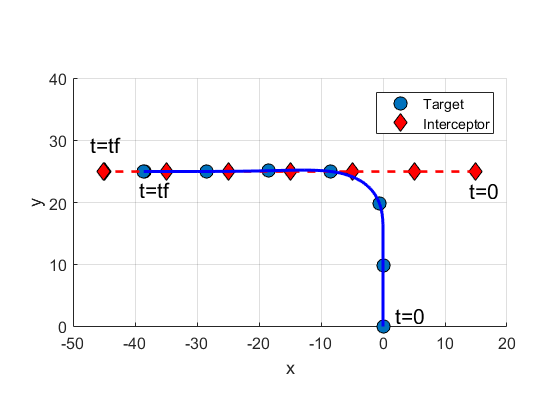
\includegraphics[width=4cm] {ptx15}}
%DIF < 		\subfigure []{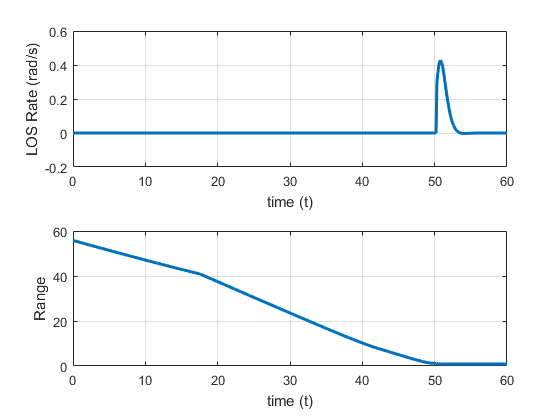
\includegraphics [width=4cm]{ptx50_range_LOSrate}}
%DIF < 		\subfigure []{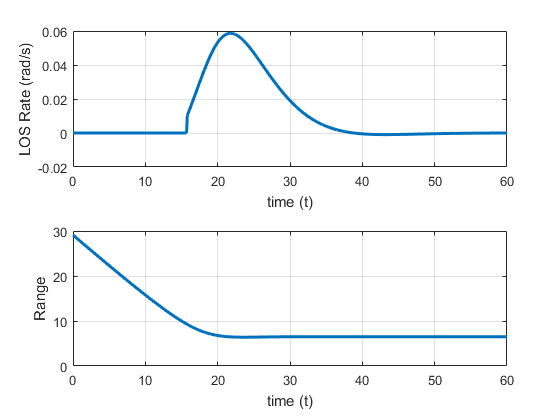
\includegraphics [width=4cm]{ptx15_range_LOSrate}}
%DIF < 		\hspace*{0mm}
%DIF < 	\end{subfigmatrix}
%DIF < 	\caption{Simulation Scenarios}
%DIF < 	\label{fig:compwithpt}
%DIF < \end{figure}
\DIFdelbegin %DIFDELCMD < 

%DIFDELCMD < %%%
\DIFdelend \begin{table}[H]
	\centering
	\caption{Traditional PN and Pseudotarget PN Following Distance and LOS rate}
	\label{my-label}
	\begin{tabular}{c|c|c|}
		\cline{2-3}
		\multicolumn{1}{l|}{}                                        & \multicolumn{1}{l|}{Following Distance} & \multicolumn{1}{l|}{Max LOS Rate (rad/s)} \\ \hline
		\multicolumn{1}{|c|}{}                                       & 0.51                                    & 0.02                                      \\ \cline{2-3} 
		\multicolumn{1}{|c|}{\multirow{-2}{*}{Traditional PN}}       & \cellcolor[HTML]{C0C0C0}                \DIFdelbeginFL \DIFdelFL{FAILED         }\DIFdelendFL & 46.07                                     \\ \hline
		\multicolumn{1}{|c|}{}                                       & 6.51                                    & 0.06                                      \\ \cline{2-3} 
		\multicolumn{1}{|c|}{\multirow{-2}{*}{PN with Pseudotarget}} & 0.88                                    & 0.04                                      \\ \hline
	\end{tabular}
\end{table}

\section{Simulations}
The \DIFdelbegin \DIFdel{pseudotarget state machine PN guidance }\DIFdelend \DIFaddbegin \DIFadd{model }\DIFaddend was validated through MATLAB simulations and a ratio for predicting following distance as a function of initial LOS, range, and sensor characteristic is presented for a non maneuvering target. Initial target conditions of $x = [-100,100]$ $y = [10,100]$ in $1$ unit increments were evaluated with a constant heading of $\beta = 180^{\circ}$. Initial uncertainty radius of the target estimate for each scenario was $0.7$ times the initial range with rate of change $dr = 1$. Interceptor initial conditions remained constant where the initial position and heading were $(0,0)$ and $90^{\circ}$ respectively. Each UAV was given the same velocity so that the speed ratio of the two vehicles was 1:1. When the interceptor's heading \DIFdelbegin \DIFdel{$\gamma = \beta$ }\DIFdelend \DIFaddbegin \DIFadd{$\gamma = 180^{\circ}$ }\DIFaddend the simulation was terminated and the \DIFdelbegin \DIFdel{final positions of the vehicles recorded }\DIFdelend \DIFaddbegin \DIFadd{range to the target was recorded as the following distance}\DIFaddend . Dividing the following distance by the initial range to the target produces a following distance initial range ratio (FDIR), shown in Equation \ref{eq:FDIR} which can be used to describe the performance of the model.



%Model validated and relationship between initial los angle, range, and sensor characteristic shown

%Non maneuvering target
% Constant heading
%Initial uncertainty radius
%dr = 1
%Interceptor guided to follow and intercept the target with highly uncertain sensor information 
%Interceptor initial conditions
%Speed ratios
%Simulation space
%Simulation end criterion
%Following distance ratio equation

% The two agent engagement model was subjected to two sets of simulations with the goal of determining a relationship between initial range and following distance. The non-maneuvering target was given a constant heading $\beta = 180^{\circ}$. The initial uncertainty radius of the target estimate for each scenario was $0.7$ times the initial range with rate of change $dr = 1$. The interceptor was tasked with intercepting and following the target based on uncertain target position estimation without entering the uncertain domain. The interceptor's initial position and heading for each simulation were $(0,0)$ and $90^{\circ}$ respectively. In the worst case scenario, the target would have equal maximum velocity as the interceptor. To evaluate the worst case, the interceptor and target were given a speed ratio of 1:1. The first set of simulations were performed for initial target position in the space $x = [-100,100]$ $y = [10,100]$ in $1$ unit increments. Once the interceptor reached a heading of $\gamma = 180^{\circ}$ the simulation was ended and the distance was recorded as following distance. For the simulation space, the ratio of following distance to initial range was calculated by Equation \ref{eq:FDIR} and the results are shown in Figure \ref{fig:Rays}.

%DIF < \begin{equation} 
%DIF < \label{eq:FDIR}
%DIF < \frac{Following Distance}{Initial Range} = FDIR
%DIF < \end{equation}
\DIFaddbegin \begin{equation} 
\DIFadd{\label{eq:FDIR}
\frac{Following Distance}{Initial Range} = FDIR
}\end{equation}
\DIFaddend 

\DIFdelbegin \begin{displaymath} 
\DIFdel{%DIFDELCMD < \label{eq:FDIR}%%%
FDIR = \sqrt{\frac{(x_{Tf}-x_{If})^2+(y_{Tf}-y_{If})^2}{(x_{T0}-x_{I0})^2+(y_{T0}-y_{I0})^2}}
}\end{displaymath}
%DIFAUXCMD
%DIFDELCMD < 

%DIFDELCMD < %%%
\DIFdelend The unit-less FDIR ratio in the simulation space is shown in the contour plot Figure \ref{fig:Rays}. Each target initial condition corresponds to a FDIR ratio on the plot, ranging from $0$ to $1.65$. FDIR is constant along each initial LOS which allows for the prediction of following distance based on initial LOS, range, and sensor $dr$. Initial LOS angles less than $45^{\circ}$ yield a FDIR ratio of near zero indicating that the following distance was near zero. Increasing LOS angles greater than $45^{\circ}$ result in progressively higher FDIR ratios indicating an increasing following distance.

% for initial LOS angles less than $45^{\circ}$ 


% The contour plot shown in Figure \ref{fig:Rays} shows 18,000 simulation results for various target initial conditions. Each target initial condition has a corresponding FDIR ratio. As expected, the following distance is near zero for initial LOS angles less than $45^{\circ}$. For initial LOS angles greater than $45^{\circ}$, the following distance increases, which is a result of the 1:1 speed ratio. The FDIR ratio is constant along each initial LOS which allows an estimate for following distance based only on initial LOS and initial range to the target. The simulations that produced Figure \ref{fig:Rays}, were for a fixed sensor rate $dr = 1$. To show how the modified PN guidance algorithm performs for a range of sensors, a second set of simulations was performed.


\begin{figure}[H]
	\centering
	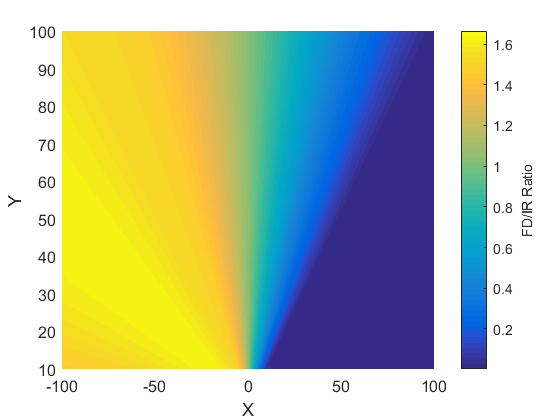
\includegraphics[width=8cm]{FDIR_Rays.png}
	\caption{\DIFdelbeginFL \DIFdelFL{Following distance to initial range ratio constant along each initial LOS}\DIFdelendFL \DIFaddbeginFL \DIFaddFL{FDIR Ratio}\DIFaddendFL }
	\label{fig:Rays}
\end{figure}

\DIFdelbegin \DIFdel{Representation }\DIFdelend \DIFaddbegin \DIFadd{A more useful representation }\DIFaddend of the models performance for a range of sensor $dr$'s is shown in Figure \ref{fig:Polar}. Simulations were performed for initial LOS angles ranging from $0^{\circ}$ to $180^{\circ}$ and sensors with $dr$ ranging from $0.5$ to $1$ in $0.5^{\circ}$ and $0.01$ unit increments respectively. Sensors with $dr < 0.5$ would not allow the interceptor to reduce the following distance much farther than the initial range for nearly all LOS angles. Sensors with $dr \geq 1$ the following distance can be reduced to nearly zero for initial LOS angles between $0$ and $45^{\circ}$. \DIFaddbegin \DIFadd{The contour polar plot was created with the help of PolarPlot3D \mbox{%DIFAUXCMD
\cite{Polar3d}}\hspace{0pt}%DIFAUXCMD
.
}\DIFaddend 

\begin{figure}[H]
	\centering
	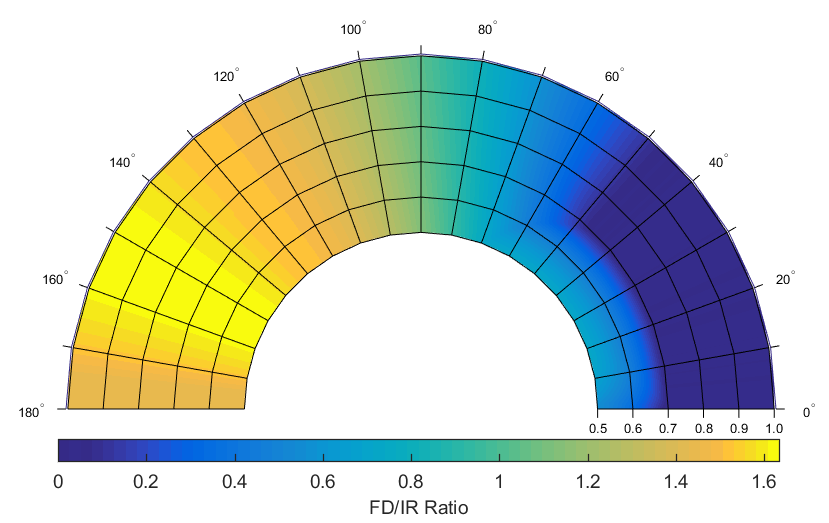
\includegraphics[width=8cm]{correctpolar.png}
	\caption{\DIFdelbeginFL \DIFdelFL{Following distance to initial range ratio for multiple sensor $dr$ confirm predicted near zero following distance for initial LOS $\leq45^\circ$}\DIFdelendFL \DIFaddbeginFL \DIFaddFL{FD/IR Rays}\DIFaddendFL }
	\label{fig:Polar}
\end{figure}

\section{Conclusion}

%What was done
% Counter UAS
% Simplified 2 agent engagement model
% interceptor estimates target position with highly uncertain sensor
% Intercepts and follow the target where vehicles have 1:1 speed ratio
% Even in worst case scenario a interceptor may reduce the following distance near zero for a limited range of initial LOS

% Future work could be a more active interceptor that attempts to close the range by flying directly towards the estimate and entering a follow in a way to minimize the following distance. 
%Implementing multi-rotor dynamics in replacement to kinematics should be done to more accurately model the engagement

% We have shown that a simplified multi-rotor UAV model equipped with on-board target sensing capabilities and guided with a pseudo-target based PN guidance system is a viable counter UAV system for a limited initial heading range. The simplified engagement model consisting of a interceptor that estimates a targets position with a highly uncertain sensor where vehicles exhibit a 1:1 speed ratio presents a worst case interception scenario. Even in worse case scenario, an interceptor may reduce the following distance near zero for a limited range of initial LOS. Future work could be a more active interceptor that attempts to close the range by flying direclty towards the estimate and entering a follow such a way to minimize the following distance for a larger range of initial LOS angles. Implementing multi-rotor dynamics in replacement to kinematics should be done to more accurately model the engagement. 


A pseudotarget based proportional navigation (PN) guidance algorithm that guides a UAV to intercept and follow a target UAV using highly uncertain sensor position information was \DIFdelbegin \DIFdel{investigated}\DIFdelend \DIFaddbegin \DIFadd{developed}\DIFaddend . Simulations were performed to \DIFdelbegin \DIFdel{determine the following distance }\DIFdelend \DIFaddbegin \DIFadd{validate the model }\DIFaddend for a finite space \DIFaddbegin \DIFadd{and a ratio for predicting following distance as a function of initial LOS, range, and sensor characteristic was presented}\DIFaddend . Near zero following distance is achievable for a finite range of initial headings and sensor $dr$'s. \DIFdelbegin %DIFDELCMD < \hl{Following distance to initial range ratios indicate that the modified guidance performs optimally when the initial LOS angle is less than $45^\circ$ and larger initial sight angles may benefit from other intercept methods.} %%%
\DIFdelend The state machine pseudotarget PN guidance algorithm was specifically designed to intercept and follow an inbound non-maneuvering target for the edge case \DIFdelbegin \DIFdel{of }\DIFdelend $1:1$ speed ratio. Initial results suggest that the proposed guidance is \DIFdelbegin \DIFdel{tracks the target with less error compared }\DIFdelend \DIFaddbegin \DIFadd{superior }\DIFaddend to traditional PN for head-on intercepts but slightly \DIFdelbegin \DIFdel{underperformed }\DIFdelend \DIFaddbegin \DIFadd{underproform }\DIFaddend in the tail-chase scenario 

\DIFaddbegin \DIFadd{Applying the guidance model presented could be applicable to the loyal wingman flight formation problem due to the models ability to approach the objective closely under high position uncertainty. 
}

\DIFaddend % Future work could involve an active interceptor that attempts to close the range by flying directly towards the estimate and entering a follow in such a way as to minimize the following distance for a larger range of initial LOS angles. Implementing multi-rotor dynamics in replacement to kinematics should be done to more accurately model the engagement. 

% It was shown that a pseudotarget based PN guidance algorithm with $wait$, $intercept$, and $follow$ states is capable of guiding a simplified multi-rotor UAV model to intercept and follow an uncertain target for a finite range of initial headings. An additional speed $1:1$ speed ratio constraint was evaluated 

% a target UAV whose position is highly uncertain for a finite range of initial headings. 

% It was shown that a multi-rotor UAV equipped with on-board target sensing capabilities and guided by a pseudotarget based PN guidance system is a viable 
%1:1 speed constraint

% It was shown that a simplified multi-rotor UAV model equipped with on-board target sensing capabilities and guided with a pseudo-target based PN guidance system is a viable counter UAV system for a limited initial heading range.

%State machine based pseudotarget (wait, intercept, and follow from behind) without entering the uncertainty region

%A pseudotarget based PN guidance algorithm for intercepting and following a target with a highly uncertain position estimate was presented.

% %Future work
% We have shown that a simplified multi-rotor UAV model equipped with on-board target sensing capabilities and guided with a pseudo-target based PN guidance system is a viable counter UAV system for a limited initial heading range. A pseudotarget based PN guidance algorithm for intercepting and following a target with a highly uncertain position estimate was presented. The pseudotarget PN algorithm operates on the principle of nulling the LOS rate between the interceptor and pseudotarget.

% The position of the pseudotarget with respect to the target estimate is determined by a state machine in three distinct states consisting of $wait$, $follow$, and $intercept$. 

% The algorithm prevents the interceptor from entering the space in which the target may exist, preventing an unintended collision, while maintaining the mission objective of intercepting and following the target. 

% A range of initial target conditions were evaluated to determine a relationship between initial target position and following distance, which lead to the realization that following distance can be expressed as a function of initial LOS and range. 

% A second set of simulations were performed to relate initial LOS angle, sensor characteristic $dr$, and range with following distance. For initial LOS angles less than $45^{\circ}$, the following distance is near zero for a range of sensor $dr$s. For initial LOS angles greater than $45^{\circ}$, the following distance increases due to the 1:1 speed ratio constraint. 

% The increase in following distance is a result of the interceptors inability to close the distance to the target. 

% Future work could involve a more active interceptor that attempts to close the range by flying directly towards the estimate and entering a follow in such a way as to minimize the following distance for a larger range of initial LOS angles. Implementing multi-rotor dynamics in replacement to kinematics should be done to more accurately model the engagement. 

\section{Acknowledgements}
The research presented was funded by Wright-Patterson Air Force Research Laboratory\DIFdelbegin \DIFdel{under SFFP }\DIFdelend \DIFaddbegin \DIFadd{. Special thanks to the sponsor of the fellowship Dr. David Grymin and Dr. David Casbeer, Dr. Eloy Garcia, and Isaac Weintraub for their recommendations during the course of this research}\DIFaddend . 


% if have a single appendix:
%\appendix[Proof of the Zonklar Equations]
% or
%\appendix  % for no appendix heading
% do not use \section anymore after \appendix, only \section*
% is possibly needed

% use appendices with more than one appendix
% then use \section to start each appendix
% you must declare a \section before using any
% \subsection or using \label (\appendices by itself
% starts a section numbered zero.)
%

% use section* for acknowledgement
%%\section*{Acknowledgment}


%%The authors would like to thank...


% Can use something like this to put references on a page
% by themselves when using endfloat and the captionsoff option.
%%\ifCLASSOPTIONcaptionsoff
%%  \newpage
%%\fi



% trigger a \newpage just before the given reference
% number - used to balance the columns on the last page
% adjust value as needed - may need to be readjusted if
% the document is modified later
%\IEEEtriggeratref{8}
% The "triggered" command can be changed if desired:
%\IEEEtriggercmd{\enlargethispage{-5in}}

% references section

% can use a bibliography generated by BibTeX as a .bbl file
% BibTeX documentation can be easily obtained at:
% http://www.ctan.org/tex-archive/biblio/bibtex/contrib/doc/
% The IEEEtran BibTeX style support page is at:
% http://www.michaelshell.org/tex/ieeetran/bibtex/
%\bibliographystyle{IEEEtran}
% argument is your BibTeX string definitions and bibliography database(s)
%\bibliography{IEEEabrv,../bib/paper}
%
% <OR> manually copy in the resultant .bbl file
% set second argument of \begin to the number of references
% (used to reserve space for the reference number labels box)

\bibliographystyle{IEEEtran}
\bibliography{bib}

\end{document}


